% Created by tikzDevice version 0.12.3.1 on 2022-09-05 10:07:29
% !TEX encoding = UTF-8 Unicode
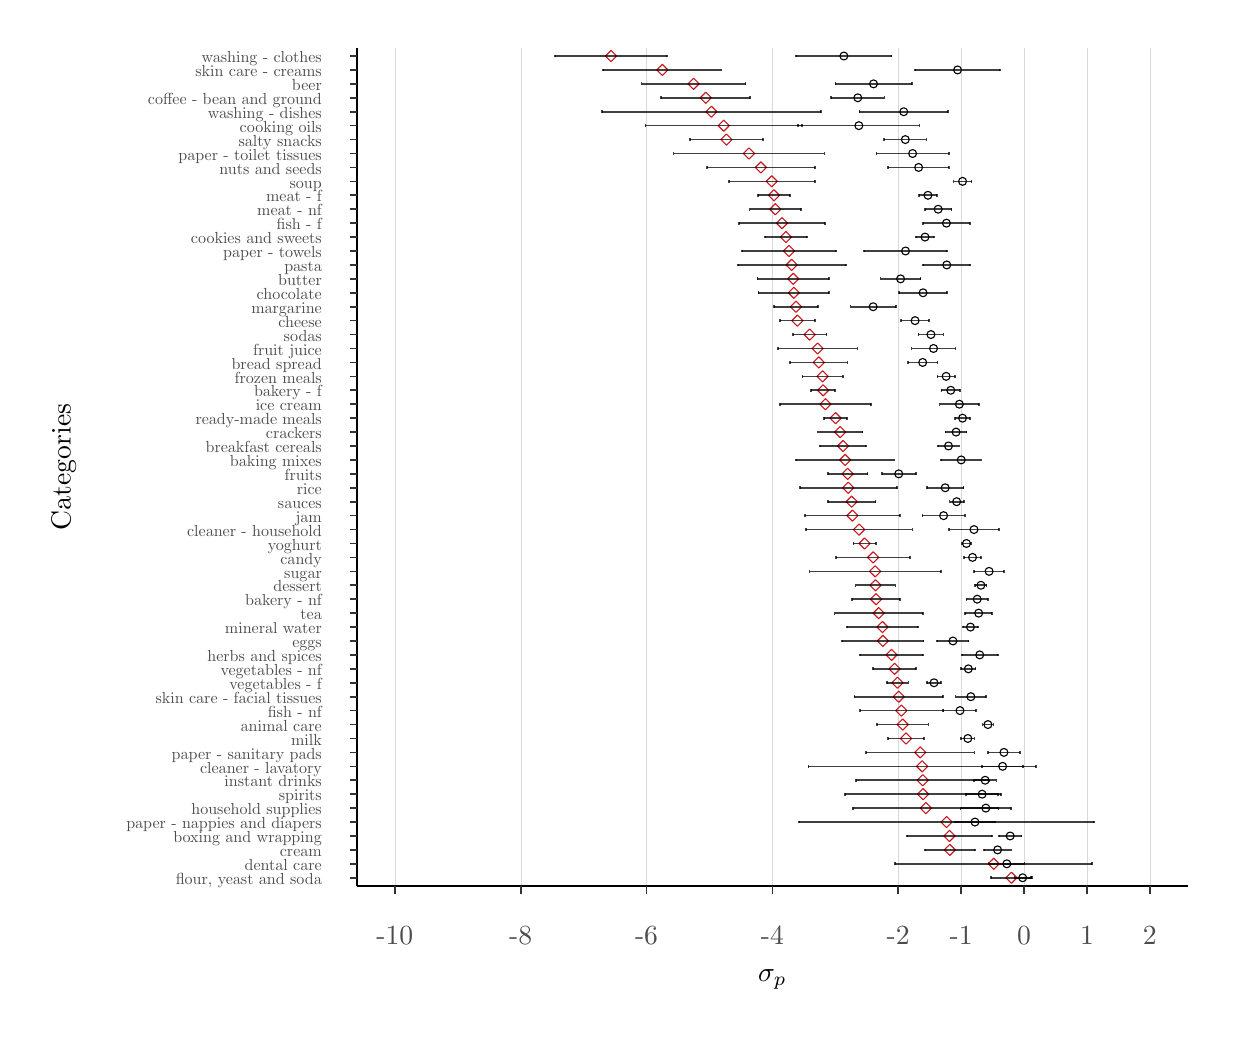
\begin{tikzpicture}[x=1pt,y=1pt]
\definecolor{fillColor}{RGB}{255,255,255}
\path[use as bounding box,fill=fillColor,fill opacity=0.00] (0,0) rectangle (433.62,361.35);
\begin{scope}
\path[clip] (  0.00,  0.00) rectangle (433.62,361.35);
\definecolor{drawColor}{RGB}{255,255,255}
\definecolor{fillColor}{RGB}{255,255,255}

\path[draw=drawColor,line width= 0.6pt,line join=round,line cap=round,fill=fillColor] (  0.00,  0.00) rectangle (433.62,361.35);
\end{scope}
\begin{scope}
\path[clip] (119.04, 51.15) rectangle (419.17,354.12);
\definecolor{drawColor}{RGB}{255,255,255}

\path[draw=drawColor,line width= 0.3pt,line join=round] (155.42, 51.15) --
	(155.42,354.12);

\path[draw=drawColor,line width= 0.3pt,line join=round] (200.89, 51.15) --
	(200.89,354.12);

\path[draw=drawColor,line width= 0.3pt,line join=round] (246.37, 51.15) --
	(246.37,354.12);

\path[draw=drawColor,line width= 0.3pt,line join=round] (291.84, 51.15) --
	(291.84,354.12);

\path[draw=drawColor,line width= 0.3pt,line join=round] (325.95, 51.15) --
	(325.95,354.12);

\path[draw=drawColor,line width= 0.3pt,line join=round] (348.68, 51.15) --
	(348.68,354.12);

\path[draw=drawColor,line width= 0.3pt,line join=round] (371.42, 51.15) --
	(371.42,354.12);

\path[draw=drawColor,line width= 0.3pt,line join=round] (394.16, 51.15) --
	(394.16,354.12);
\definecolor{drawColor}{gray}{0.85}

\path[draw=drawColor,line width= 0.1pt,line join=round] (132.68, 51.15) --
	(132.68,354.12);

\path[draw=drawColor,line width= 0.1pt,line join=round] (178.16, 51.15) --
	(178.16,354.12);

\path[draw=drawColor,line width= 0.1pt,line join=round] (223.63, 51.15) --
	(223.63,354.12);

\path[draw=drawColor,line width= 0.1pt,line join=round] (269.10, 51.15) --
	(269.10,354.12);

\path[draw=drawColor,line width= 0.1pt,line join=round] (314.58, 51.15) --
	(314.58,354.12);

\path[draw=drawColor,line width= 0.1pt,line join=round] (337.31, 51.15) --
	(337.31,354.12);

\path[draw=drawColor,line width= 0.1pt,line join=round] (360.05, 51.15) --
	(360.05,354.12);

\path[draw=drawColor,line width= 0.1pt,line join=round] (382.79, 51.15) --
	(382.79,354.12);

\path[draw=drawColor,line width= 0.1pt,line join=round] (405.52, 51.15) --
	(405.52,354.12);
\definecolor{drawColor}{RGB}{0,0,0}

\path[draw=drawColor,line width= 0.4pt,line join=round,line cap=round] (346.98,109.53) circle (  1.43);

\path[draw=drawColor,line width= 0.4pt,line join=round,line cap=round] (333.56,230.32) circle (  1.43);

\path[draw=drawColor,line width= 0.4pt,line join=round,line cap=round] (343.12,154.83) circle (  1.43);

\path[draw=drawColor,line width= 0.4pt,line join=round,line cap=round] (337.33,205.15) circle (  1.43);

\path[draw=drawColor,line width= 0.4pt,line join=round,line cap=round] (305.65,341.04) circle (  1.43);

\path[draw=drawColor,line width= 0.4pt,line join=round,line cap=round] (355.02, 69.27) circle (  1.43);

\path[draw=drawColor,line width= 0.4pt,line join=round,line cap=round] (323.40,240.38) circle (  1.43);

\path[draw=drawColor,line width= 0.4pt,line join=round,line cap=round] (332.74,210.19) circle (  1.43);

\path[draw=drawColor,line width= 0.4pt,line join=round,line cap=round] (315.42,270.58) circle (  1.43);

\path[draw=drawColor,line width= 0.4pt,line join=round,line cap=round] (341.42,169.93) circle (  1.43);

\path[draw=drawColor,line width= 0.4pt,line join=round,line cap=round] (320.66,255.48) circle (  1.43);

\path[draw=drawColor,line width= 0.4pt,line join=round,line cap=round] (323.54,265.55) circle (  1.43);

\path[draw=drawColor,line width= 0.4pt,line join=round,line cap=round] (341.95,179.99) circle (  1.43);

\path[draw=drawColor,line width= 0.4pt,line join=round,line cap=round] (352.30, 94.43) circle (  1.43);

\path[draw=drawColor,line width= 0.4pt,line join=round,line cap=round] (299.96,336.01) circle (  1.43);

\path[draw=drawColor,line width= 0.4pt,line join=round,line cap=round] (324.26,285.68) circle (  1.43);

\path[draw=drawColor,line width= 0.4pt,line join=round,line cap=round] (300.34,325.94) circle (  1.43);

\path[draw=drawColor,line width= 0.4pt,line join=round,line cap=round] (335.47,215.22) circle (  1.43);

\path[draw=drawColor,line width= 0.4pt,line join=round,line cap=round] (350.48, 64.24) circle (  1.43);

\path[draw=drawColor,line width= 0.4pt,line join=round,line cap=round] (353.81, 59.21) circle (  1.43);

\path[draw=drawColor,line width= 0.4pt,line join=round,line cap=round] (344.46,159.86) circle (  1.43);

\path[draw=drawColor,line width= 0.4pt,line join=round,line cap=round] (334.35,139.73) circle (  1.43);

\path[draw=drawColor,line width= 0.4pt,line join=round,line cap=round] (331.99,290.71) circle (  1.43);

\path[draw=drawColor,line width= 0.4pt,line join=round,line cap=round] (336.88,114.57) circle (  1.43);

\path[draw=drawColor,line width= 0.4pt,line join=round,line cap=round] (359.54, 54.17) circle (  1.43);

\path[draw=drawColor,line width= 0.4pt,line join=round,line cap=round] (331.88,235.35) circle (  1.43);

\path[draw=drawColor,line width= 0.4pt,line join=round,line cap=round] (327.32,245.42) circle (  1.43);

\path[draw=drawColor,line width= 0.4pt,line join=round,line cap=round] (314.75,200.12) circle (  1.43);

\path[draw=drawColor,line width= 0.4pt,line join=round,line cap=round] (344.02,134.70) circle (  1.43);

\path[draw=drawColor,line width= 0.4pt,line join=round,line cap=round] (346.22, 79.34) circle (  1.43);

\path[draw=drawColor,line width= 0.4pt,line join=round,line cap=round] (336.67,225.29) circle (  1.43);

\path[draw=drawColor,line width= 0.4pt,line join=round,line cap=round] (345.98, 89.40) circle (  1.43);

\path[draw=drawColor,line width= 0.4pt,line join=round,line cap=round] (330.96,185.02) circle (  1.43);

\path[draw=drawColor,line width= 0.4pt,line join=round,line cap=round] (305.50,260.51) circle (  1.43);

\path[draw=drawColor,line width= 0.4pt,line join=round,line cap=round] (325.31,300.78) circle (  1.43);

\path[draw=drawColor,line width= 0.4pt,line join=round,line cap=round] (329.00,295.74) circle (  1.43);

\path[draw=drawColor,line width= 0.4pt,line join=round,line cap=round] (339.73,104.50) circle (  1.43);

\path[draw=drawColor,line width= 0.4pt,line join=round,line cap=round] (340.67,144.76) circle (  1.43);

\path[draw=drawColor,line width= 0.4pt,line join=round,line cap=round] (321.94,310.84) circle (  1.43);

\path[draw=drawColor,line width= 0.4pt,line join=round,line cap=round] (342.30, 74.30) circle (  1.43);

\path[draw=drawColor,line width= 0.4pt,line join=round,line cap=round] (352.77, 99.47) circle (  1.43);

\path[draw=drawColor,line width= 0.4pt,line join=round,line cap=round] (319.77,315.87) circle (  1.43);

\path[draw=drawColor,line width= 0.4pt,line join=round,line cap=round] (317.21,280.65) circle (  1.43);

\path[draw=drawColor,line width= 0.4pt,line join=round,line cap=round] (332.11,275.61) circle (  1.43);

\path[draw=drawColor,line width= 0.4pt,line join=round,line cap=round] (337.81,220.25) circle (  1.43);

\path[draw=drawColor,line width= 0.4pt,line join=round,line cap=round] (331.55,195.09) circle (  1.43);

\path[draw=drawColor,line width= 0.4pt,line join=round,line cap=round] (317.13,320.91) circle (  1.43);

\path[draw=drawColor,line width= 0.4pt,line join=round,line cap=round] (335.68,190.06) circle (  1.43);

\path[draw=drawColor,line width= 0.4pt,line join=round,line cap=round] (336.01,346.07) circle (  1.43);

\path[draw=drawColor,line width= 0.4pt,line join=round,line cap=round] (340.82,119.60) circle (  1.43);

\path[draw=drawColor,line width= 0.4pt,line join=round,line cap=round] (326.39,250.45) circle (  1.43);

\path[draw=drawColor,line width= 0.4pt,line join=round,line cap=round] (337.81,305.81) circle (  1.43);

\path[draw=drawColor,line width= 0.4pt,line join=round,line cap=round] (344.89, 84.37) circle (  1.43);

\path[draw=drawColor,line width= 0.4pt,line join=round,line cap=round] (347.40,164.89) circle (  1.43);

\path[draw=drawColor,line width= 0.4pt,line join=round,line cap=round] (343.64,149.79) circle (  1.43);

\path[draw=drawColor,line width= 0.4pt,line join=round,line cap=round] (327.50,124.63) circle (  1.43);

\path[draw=drawColor,line width= 0.4pt,line join=round,line cap=round] (339.91,129.66) circle (  1.43);

\path[draw=drawColor,line width= 0.4pt,line join=round,line cap=round] (294.93,351.10) circle (  1.43);

\path[draw=drawColor,line width= 0.4pt,line join=round,line cap=round] (316.57,330.97) circle (  1.43);

\path[draw=drawColor,line width= 0.4pt,line join=round,line cap=round] (339.23,174.96) circle (  1.43);
\definecolor{drawColor}{RGB}{0,0,0}

\path[draw=drawColor,draw opacity=0.75,line width= 0.6pt,line join=round] (348.94,109.03) --
	(348.94,110.04);

\path[draw=drawColor,draw opacity=0.75,line width= 0.6pt,line join=round] (348.94,109.53) --
	(345.03,109.53);

\path[draw=drawColor,draw opacity=0.75,line width= 0.6pt,line join=round] (345.03,109.03) --
	(345.03,110.04);

\path[draw=drawColor,draw opacity=0.75,line width= 0.6pt,line join=round] (336.97,229.81) --
	(336.97,230.82);

\path[draw=drawColor,draw opacity=0.75,line width= 0.6pt,line join=round] (336.97,230.32) --
	(330.15,230.32);

\path[draw=drawColor,draw opacity=0.75,line width= 0.6pt,line join=round] (330.15,229.81) --
	(330.15,230.82);

\path[draw=drawColor,draw opacity=0.75,line width= 0.6pt,line join=round] (347.02,154.32) --
	(347.02,155.33);

\path[draw=drawColor,draw opacity=0.75,line width= 0.6pt,line join=round] (347.02,154.83) --
	(339.22,154.83);

\path[draw=drawColor,draw opacity=0.75,line width= 0.6pt,line join=round] (339.22,154.32) --
	(339.22,155.33);

\path[draw=drawColor,draw opacity=0.75,line width= 0.6pt,line join=round] (344.60,204.65) --
	(344.60,205.66);

\path[draw=drawColor,draw opacity=0.75,line width= 0.6pt,line join=round] (344.60,205.15) --
	(330.07,205.15);

\path[draw=drawColor,draw opacity=0.75,line width= 0.6pt,line join=round] (330.07,204.65) --
	(330.07,205.66);

\path[draw=drawColor,draw opacity=0.75,line width= 0.6pt,line join=round] (319.43,340.53) --
	(319.43,341.54);

\path[draw=drawColor,draw opacity=0.75,line width= 0.6pt,line join=round] (319.43,341.04) --
	(291.87,341.04);

\path[draw=drawColor,draw opacity=0.75,line width= 0.6pt,line join=round] (291.87,340.53) --
	(291.87,341.54);

\path[draw=drawColor,draw opacity=0.75,line width= 0.6pt,line join=round] (359.12, 68.77) --
	(359.12, 69.77);

\path[draw=drawColor,draw opacity=0.75,line width= 0.6pt,line join=round] (359.12, 69.27) --
	(350.93, 69.27);

\path[draw=drawColor,draw opacity=0.75,line width= 0.6pt,line join=round] (350.93, 68.77) --
	(350.93, 69.77);

\path[draw=drawColor,draw opacity=0.75,line width= 0.6pt,line join=round] (328.80,239.88) --
	(328.80,240.89);

\path[draw=drawColor,draw opacity=0.75,line width= 0.6pt,line join=round] (328.80,240.38) --
	(318.00,240.38);

\path[draw=drawColor,draw opacity=0.75,line width= 0.6pt,line join=round] (318.00,239.88) --
	(318.00,240.89);

\path[draw=drawColor,draw opacity=0.75,line width= 0.6pt,line join=round] (336.65,209.68) --
	(336.65,210.69);

\path[draw=drawColor,draw opacity=0.75,line width= 0.6pt,line join=round] (336.65,210.19) --
	(328.83,210.19);

\path[draw=drawColor,draw opacity=0.75,line width= 0.6pt,line join=round] (328.83,209.68) --
	(328.83,210.69);

\path[draw=drawColor,draw opacity=0.75,line width= 0.6pt,line join=round] (322.64,270.08) --
	(322.64,271.08);

\path[draw=drawColor,draw opacity=0.75,line width= 0.6pt,line join=round] (322.64,270.58) --
	(308.21,270.58);

\path[draw=drawColor,draw opacity=0.75,line width= 0.6pt,line join=round] (308.21,270.08) --
	(308.21,271.08);

\path[draw=drawColor,draw opacity=0.75,line width= 0.6pt,line join=round] (344.52,169.42) --
	(344.52,170.43);

\path[draw=drawColor,draw opacity=0.75,line width= 0.6pt,line join=round] (344.52,169.93) --
	(338.32,169.93);

\path[draw=drawColor,draw opacity=0.75,line width= 0.6pt,line join=round] (338.32,169.42) --
	(338.32,170.43);

\path[draw=drawColor,draw opacity=0.75,line width= 0.6pt,line join=round] (325.75,254.98) --
	(325.75,255.99);

\path[draw=drawColor,draw opacity=0.75,line width= 0.6pt,line join=round] (325.75,255.48) --
	(315.56,255.48);

\path[draw=drawColor,draw opacity=0.75,line width= 0.6pt,line join=round] (315.56,254.98) --
	(315.56,255.99);

\path[draw=drawColor,draw opacity=0.75,line width= 0.6pt,line join=round] (332.11,265.04) --
	(332.11,266.05);

\path[draw=drawColor,draw opacity=0.75,line width= 0.6pt,line join=round] (332.11,265.55) --
	(314.96,265.55);

\path[draw=drawColor,draw opacity=0.75,line width= 0.6pt,line join=round] (314.96,265.04) --
	(314.96,266.05);

\path[draw=drawColor,draw opacity=0.75,line width= 0.6pt,line join=round] (350.91,179.49) --
	(350.91,180.49);

\path[draw=drawColor,draw opacity=0.75,line width= 0.6pt,line join=round] (350.91,179.99) --
	(332.99,179.99);

\path[draw=drawColor,draw opacity=0.75,line width= 0.6pt,line join=round] (332.99,179.49) --
	(332.99,180.49);

\path[draw=drawColor,draw opacity=0.75,line width= 0.6pt,line join=round] (359.66, 93.93) --
	(359.66, 94.94);

\path[draw=drawColor,draw opacity=0.75,line width= 0.6pt,line join=round] (359.66, 94.43) --
	(344.95, 94.43);

\path[draw=drawColor,draw opacity=0.75,line width= 0.6pt,line join=round] (344.95, 93.93) --
	(344.95, 94.94);

\path[draw=drawColor,draw opacity=0.75,line width= 0.6pt,line join=round] (309.58,335.50) --
	(309.58,336.51);

\path[draw=drawColor,draw opacity=0.75,line width= 0.6pt,line join=round] (309.58,336.01) --
	(290.33,336.01);

\path[draw=drawColor,draw opacity=0.75,line width= 0.6pt,line join=round] (290.33,335.50) --
	(290.33,336.51);

\path[draw=drawColor,draw opacity=0.75,line width= 0.6pt,line join=round] (327.50,285.17) --
	(327.50,286.18);

\path[draw=drawColor,draw opacity=0.75,line width= 0.6pt,line join=round] (327.50,285.68) --
	(321.02,285.68);

\path[draw=drawColor,draw opacity=0.75,line width= 0.6pt,line join=round] (321.02,285.17) --
	(321.02,286.18);

\path[draw=drawColor,draw opacity=0.75,line width= 0.6pt,line join=round] (322.22,325.44) --
	(322.22,326.44);

\path[draw=drawColor,draw opacity=0.75,line width= 0.6pt,line join=round] (322.22,325.94) --
	(278.46,325.94);

\path[draw=drawColor,draw opacity=0.75,line width= 0.6pt,line join=round] (278.46,325.44) --
	(278.46,326.44);

\path[draw=drawColor,draw opacity=0.75,line width= 0.6pt,line join=round] (339.29,214.72) --
	(339.29,215.72);

\path[draw=drawColor,draw opacity=0.75,line width= 0.6pt,line join=round] (339.29,215.22) --
	(331.64,215.22);

\path[draw=drawColor,draw opacity=0.75,line width= 0.6pt,line join=round] (331.64,214.72) --
	(331.64,215.72);

\path[draw=drawColor,draw opacity=0.75,line width= 0.6pt,line join=round] (355.46, 63.74) --
	(355.46, 64.74);

\path[draw=drawColor,draw opacity=0.75,line width= 0.6pt,line join=round] (355.46, 64.24) --
	(345.50, 64.24);

\path[draw=drawColor,draw opacity=0.75,line width= 0.6pt,line join=round] (345.50, 63.74) --
	(345.50, 64.74);

\path[draw=drawColor,draw opacity=0.75,line width= 0.6pt,line join=round] (360.18, 58.70) --
	(360.18, 59.71);

\path[draw=drawColor,draw opacity=0.75,line width= 0.6pt,line join=round] (360.18, 59.21) --
	(347.43, 59.21);

\path[draw=drawColor,draw opacity=0.75,line width= 0.6pt,line join=round] (347.43, 58.70) --
	(347.43, 59.71);

\path[draw=drawColor,draw opacity=0.75,line width= 0.6pt,line join=round] (346.49,159.36) --
	(346.49,160.36);

\path[draw=drawColor,draw opacity=0.75,line width= 0.6pt,line join=round] (346.49,159.86) --
	(342.43,159.86);

\path[draw=drawColor,draw opacity=0.75,line width= 0.6pt,line join=round] (342.43,159.36) --
	(342.43,160.36);

\path[draw=drawColor,draw opacity=0.75,line width= 0.6pt,line join=round] (340.02,139.23) --
	(340.02,140.23);

\path[draw=drawColor,draw opacity=0.75,line width= 0.6pt,line join=round] (340.02,139.73) --
	(328.69,139.73);

\path[draw=drawColor,draw opacity=0.75,line width= 0.6pt,line join=round] (328.69,139.23) --
	(328.69,140.23);

\path[draw=drawColor,draw opacity=0.75,line width= 0.6pt,line join=round] (340.47,290.21) --
	(340.47,291.21);

\path[draw=drawColor,draw opacity=0.75,line width= 0.6pt,line join=round] (340.47,290.71) --
	(323.50,290.71);

\path[draw=drawColor,draw opacity=0.75,line width= 0.6pt,line join=round] (323.50,290.21) --
	(323.50,291.21);

\path[draw=drawColor,draw opacity=0.75,line width= 0.6pt,line join=round] (342.79,114.06) --
	(342.79,115.07);

\path[draw=drawColor,draw opacity=0.75,line width= 0.6pt,line join=round] (342.79,114.57) --
	(330.98,114.57);

\path[draw=drawColor,draw opacity=0.75,line width= 0.6pt,line join=round] (330.98,114.06) --
	(330.98,115.07);

\path[draw=drawColor,draw opacity=0.75,line width= 0.6pt,line join=round] (362.53, 53.67) --
	(362.53, 54.68);

\path[draw=drawColor,draw opacity=0.75,line width= 0.6pt,line join=round] (362.53, 54.17) --
	(356.55, 54.17);

\path[draw=drawColor,draw opacity=0.75,line width= 0.6pt,line join=round] (356.55, 53.67) --
	(356.55, 54.68);

\path[draw=drawColor,draw opacity=0.75,line width= 0.6pt,line join=round] (335.07,234.85) --
	(335.07,235.85);

\path[draw=drawColor,draw opacity=0.75,line width= 0.6pt,line join=round] (335.07,235.35) --
	(328.70,235.35);

\path[draw=drawColor,draw opacity=0.75,line width= 0.6pt,line join=round] (328.70,234.85) --
	(328.70,235.85);

\path[draw=drawColor,draw opacity=0.75,line width= 0.6pt,line join=round] (335.26,244.91) --
	(335.26,245.92);

\path[draw=drawColor,draw opacity=0.75,line width= 0.6pt,line join=round] (335.26,245.42) --
	(319.38,245.42);

\path[draw=drawColor,draw opacity=0.75,line width= 0.6pt,line join=round] (319.38,244.91) --
	(319.38,245.92);

\path[draw=drawColor,draw opacity=0.75,line width= 0.6pt,line join=round] (320.88,199.62) --
	(320.88,200.63);

\path[draw=drawColor,draw opacity=0.75,line width= 0.6pt,line join=round] (320.88,200.12) --
	(308.62,200.12);

\path[draw=drawColor,draw opacity=0.75,line width= 0.6pt,line join=round] (308.62,199.62) --
	(308.62,200.63);

\path[draw=drawColor,draw opacity=0.75,line width= 0.6pt,line join=round] (350.52,134.19) --
	(350.52,135.20);

\path[draw=drawColor,draw opacity=0.75,line width= 0.6pt,line join=round] (350.52,134.70) --
	(337.53,134.70);

\path[draw=drawColor,draw opacity=0.75,line width= 0.6pt,line join=round] (337.53,134.19) --
	(337.53,135.20);

\path[draw=drawColor,draw opacity=0.75,line width= 0.6pt,line join=round] (355.35, 78.83) --
	(355.35, 79.84);

\path[draw=drawColor,draw opacity=0.75,line width= 0.6pt,line join=round] (355.35, 79.34) --
	(337.08, 79.34);

\path[draw=drawColor,draw opacity=0.75,line width= 0.6pt,line join=round] (337.08, 78.83) --
	(337.08, 79.84);

\path[draw=drawColor,draw opacity=0.75,line width= 0.6pt,line join=round] (343.84,224.78) --
	(343.84,225.79);

\path[draw=drawColor,draw opacity=0.75,line width= 0.6pt,line join=round] (343.84,225.29) --
	(329.51,225.29);

\path[draw=drawColor,draw opacity=0.75,line width= 0.6pt,line join=round] (329.51,224.78) --
	(329.51,225.79);

\path[draw=drawColor,draw opacity=0.75,line width= 0.6pt,line join=round] (350.07, 88.90) --
	(350.07, 89.91);

\path[draw=drawColor,draw opacity=0.75,line width= 0.6pt,line join=round] (350.07, 89.40) --
	(341.90, 89.40);

\path[draw=drawColor,draw opacity=0.75,line width= 0.6pt,line join=round] (341.90, 88.90) --
	(341.90, 89.91);

\path[draw=drawColor,draw opacity=0.75,line width= 0.6pt,line join=round] (338.61,184.52) --
	(338.61,185.53);

\path[draw=drawColor,draw opacity=0.75,line width= 0.6pt,line join=round] (338.61,185.02) --
	(323.32,185.02);

\path[draw=drawColor,draw opacity=0.75,line width= 0.6pt,line join=round] (323.32,184.52) --
	(323.32,185.53);

\path[draw=drawColor,draw opacity=0.75,line width= 0.6pt,line join=round] (313.68,260.01) --
	(313.68,261.02);

\path[draw=drawColor,draw opacity=0.75,line width= 0.6pt,line join=round] (313.68,260.51) --
	(297.33,260.51);

\path[draw=drawColor,draw opacity=0.75,line width= 0.6pt,line join=round] (297.33,260.01) --
	(297.33,261.02);

\path[draw=drawColor,draw opacity=0.75,line width= 0.6pt,line join=round] (328.53,300.27) --
	(328.53,301.28);

\path[draw=drawColor,draw opacity=0.75,line width= 0.6pt,line join=round] (328.53,300.78) --
	(322.09,300.78);

\path[draw=drawColor,draw opacity=0.75,line width= 0.6pt,line join=round] (322.09,300.27) --
	(322.09,301.28);

\path[draw=drawColor,draw opacity=0.75,line width= 0.6pt,line join=round] (333.83,295.24) --
	(333.83,296.25);

\path[draw=drawColor,draw opacity=0.75,line width= 0.6pt,line join=round] (333.83,295.74) --
	(324.17,295.74);

\path[draw=drawColor,draw opacity=0.75,line width= 0.6pt,line join=round] (324.17,295.24) --
	(324.17,296.25);

\path[draw=drawColor,draw opacity=0.75,line width= 0.6pt,line join=round] (342.11,104.00) --
	(342.11,105.00);

\path[draw=drawColor,draw opacity=0.75,line width= 0.6pt,line join=round] (342.11,104.50) --
	(337.35,104.50);

\path[draw=drawColor,draw opacity=0.75,line width= 0.6pt,line join=round] (337.35,104.00) --
	(337.35,105.00);

\path[draw=drawColor,draw opacity=0.75,line width= 0.6pt,line join=round] (343.49,144.26) --
	(343.49,145.27);

\path[draw=drawColor,draw opacity=0.75,line width= 0.6pt,line join=round] (343.49,144.76) --
	(337.86,144.76);

\path[draw=drawColor,draw opacity=0.75,line width= 0.6pt,line join=round] (337.86,144.26) --
	(337.86,145.27);

\path[draw=drawColor,draw opacity=0.75,line width= 0.6pt,line join=round] (333.01,310.34) --
	(333.01,311.34);

\path[draw=drawColor,draw opacity=0.75,line width= 0.6pt,line join=round] (333.01,310.84) --
	(310.88,310.84);

\path[draw=drawColor,draw opacity=0.75,line width= 0.6pt,line join=round] (310.88,310.34) --
	(310.88,311.34);

\path[draw=drawColor,draw opacity=0.75,line width= 0.6pt,line join=round] (349.49, 73.80) --
	(349.49, 74.81);

\path[draw=drawColor,draw opacity=0.75,line width= 0.6pt,line join=round] (349.49, 74.30) --
	(335.12, 74.30);

\path[draw=drawColor,draw opacity=0.75,line width= 0.6pt,line join=round] (335.12, 73.80) --
	(335.12, 74.81);

\path[draw=drawColor,draw opacity=0.75,line width= 0.6pt,line join=round] (358.47, 98.96) --
	(358.47, 99.97);

\path[draw=drawColor,draw opacity=0.75,line width= 0.6pt,line join=round] (358.47, 99.47) --
	(347.08, 99.47);

\path[draw=drawColor,draw opacity=0.75,line width= 0.6pt,line join=round] (347.08, 98.96) --
	(347.08, 99.97);

\path[draw=drawColor,draw opacity=0.75,line width= 0.6pt,line join=round] (332.85,315.37) --
	(332.85,316.38);

\path[draw=drawColor,draw opacity=0.75,line width= 0.6pt,line join=round] (332.85,315.87) --
	(306.68,315.87);

\path[draw=drawColor,draw opacity=0.75,line width= 0.6pt,line join=round] (306.68,315.37) --
	(306.68,316.38);

\path[draw=drawColor,draw opacity=0.75,line width= 0.6pt,line join=round] (332.31,280.14) --
	(332.31,281.15);

\path[draw=drawColor,draw opacity=0.75,line width= 0.6pt,line join=round] (332.31,280.65) --
	(302.12,280.65);

\path[draw=drawColor,draw opacity=0.75,line width= 0.6pt,line join=round] (302.12,280.14) --
	(302.12,281.15);

\path[draw=drawColor,draw opacity=0.75,line width= 0.6pt,line join=round] (340.59,275.11) --
	(340.59,276.12);

\path[draw=drawColor,draw opacity=0.75,line width= 0.6pt,line join=round] (340.59,275.61) --
	(323.63,275.61);

\path[draw=drawColor,draw opacity=0.75,line width= 0.6pt,line join=round] (323.63,275.11) --
	(323.63,276.12);

\path[draw=drawColor,draw opacity=0.75,line width= 0.6pt,line join=round] (340.52,219.75) --
	(340.52,220.76);

\path[draw=drawColor,draw opacity=0.75,line width= 0.6pt,line join=round] (340.52,220.25) --
	(335.10,220.25);

\path[draw=drawColor,draw opacity=0.75,line width= 0.6pt,line join=round] (335.10,219.75) --
	(335.10,220.76);

\path[draw=drawColor,draw opacity=0.75,line width= 0.6pt,line join=round] (338.16,194.59) --
	(338.16,195.59);

\path[draw=drawColor,draw opacity=0.75,line width= 0.6pt,line join=round] (338.16,195.09) --
	(324.94,195.09);

\path[draw=drawColor,draw opacity=0.75,line width= 0.6pt,line join=round] (324.94,194.59) --
	(324.94,195.59);

\path[draw=drawColor,draw opacity=0.75,line width= 0.6pt,line join=round] (324.75,320.40) --
	(324.75,321.41);

\path[draw=drawColor,draw opacity=0.75,line width= 0.6pt,line join=round] (324.75,320.91) --
	(309.51,320.91);

\path[draw=drawColor,draw opacity=0.75,line width= 0.6pt,line join=round] (309.51,320.40) --
	(309.51,321.41);

\path[draw=drawColor,draw opacity=0.75,line width= 0.6pt,line join=round] (338.24,189.55) --
	(338.24,190.56);

\path[draw=drawColor,draw opacity=0.75,line width= 0.6pt,line join=round] (338.24,190.06) --
	(333.11,190.06);

\path[draw=drawColor,draw opacity=0.75,line width= 0.6pt,line join=round] (333.11,189.55) --
	(333.11,190.56);

\path[draw=drawColor,draw opacity=0.75,line width= 0.6pt,line join=round] (351.36,345.57) --
	(351.36,346.57);

\path[draw=drawColor,draw opacity=0.75,line width= 0.6pt,line join=round] (351.36,346.07) --
	(320.66,346.07);

\path[draw=drawColor,draw opacity=0.75,line width= 0.6pt,line join=round] (320.66,345.57) --
	(320.66,346.57);

\path[draw=drawColor,draw opacity=0.75,line width= 0.6pt,line join=round] (346.32,119.10) --
	(346.32,120.10);

\path[draw=drawColor,draw opacity=0.75,line width= 0.6pt,line join=round] (346.32,119.60) --
	(335.31,119.60);

\path[draw=drawColor,draw opacity=0.75,line width= 0.6pt,line join=round] (335.31,119.10) --
	(335.31,120.10);

\path[draw=drawColor,draw opacity=0.75,line width= 0.6pt,line join=round] (330.91,249.95) --
	(330.91,250.95);

\path[draw=drawColor,draw opacity=0.75,line width= 0.6pt,line join=round] (330.91,250.45) --
	(321.87,250.45);

\path[draw=drawColor,draw opacity=0.75,line width= 0.6pt,line join=round] (321.87,249.95) --
	(321.87,250.95);

\path[draw=drawColor,draw opacity=0.75,line width= 0.6pt,line join=round] (341.07,305.31) --
	(341.07,306.31);

\path[draw=drawColor,draw opacity=0.75,line width= 0.6pt,line join=round] (341.07,305.81) --
	(334.55,305.81);

\path[draw=drawColor,draw opacity=0.75,line width= 0.6pt,line join=round] (334.55,305.31) --
	(334.55,306.31);

\path[draw=drawColor,draw opacity=0.75,line width= 0.6pt,line join=round] (350.73, 83.87) --
	(350.73, 84.87);

\path[draw=drawColor,draw opacity=0.75,line width= 0.6pt,line join=round] (350.73, 84.37) --
	(339.05, 84.37);

\path[draw=drawColor,draw opacity=0.75,line width= 0.6pt,line join=round] (339.05, 83.87) --
	(339.05, 84.87);

\path[draw=drawColor,draw opacity=0.75,line width= 0.6pt,line join=round] (352.84,164.39) --
	(352.84,165.40);

\path[draw=drawColor,draw opacity=0.75,line width= 0.6pt,line join=round] (352.84,164.89) --
	(341.96,164.89);

\path[draw=drawColor,draw opacity=0.75,line width= 0.6pt,line join=round] (341.96,164.39) --
	(341.96,165.40);

\path[draw=drawColor,draw opacity=0.75,line width= 0.6pt,line join=round] (348.52,149.29) --
	(348.52,150.30);

\path[draw=drawColor,draw opacity=0.75,line width= 0.6pt,line join=round] (348.52,149.79) --
	(338.76,149.79);

\path[draw=drawColor,draw opacity=0.75,line width= 0.6pt,line join=round] (338.76,149.29) --
	(338.76,150.30);

\path[draw=drawColor,draw opacity=0.75,line width= 0.6pt,line join=round] (330.00,124.13) --
	(330.00,125.13);

\path[draw=drawColor,draw opacity=0.75,line width= 0.6pt,line join=round] (330.00,124.63) --
	(325.01,124.63);

\path[draw=drawColor,draw opacity=0.75,line width= 0.6pt,line join=round] (325.01,124.13) --
	(325.01,125.13);

\path[draw=drawColor,draw opacity=0.75,line width= 0.6pt,line join=round] (342.53,129.16) --
	(342.53,130.17);

\path[draw=drawColor,draw opacity=0.75,line width= 0.6pt,line join=round] (342.53,129.66) --
	(337.30,129.66);

\path[draw=drawColor,draw opacity=0.75,line width= 0.6pt,line join=round] (337.30,129.16) --
	(337.30,130.17);

\path[draw=drawColor,draw opacity=0.75,line width= 0.6pt,line join=round] (312.14,350.60) --
	(312.14,351.61);

\path[draw=drawColor,draw opacity=0.75,line width= 0.6pt,line join=round] (312.14,351.10) --
	(277.73,351.10);

\path[draw=drawColor,draw opacity=0.75,line width= 0.6pt,line join=round] (277.73,350.60) --
	(277.73,351.61);

\path[draw=drawColor,draw opacity=0.75,line width= 0.6pt,line join=round] (332.59,330.47) --
	(332.59,331.48);

\path[draw=drawColor,draw opacity=0.75,line width= 0.6pt,line join=round] (332.59,330.97) --
	(300.55,330.97);

\path[draw=drawColor,draw opacity=0.75,line width= 0.6pt,line join=round] (300.55,330.47) --
	(300.55,331.48);

\path[draw=drawColor,draw opacity=0.75,line width= 0.6pt,line join=round] (340.86,174.46) --
	(340.86,175.46);

\path[draw=drawColor,draw opacity=0.75,line width= 0.6pt,line join=round] (340.86,174.96) --
	(337.59,174.96);

\path[draw=drawColor,draw opacity=0.75,line width= 0.6pt,line join=round] (337.59,174.46) --
	(337.59,175.46);
\definecolor{drawColor}{RGB}{203,24,29}

\path[draw=drawColor,line width= 0.4pt,line join=round,line cap=round] (314.17,109.53) --
	(316.19,111.55) --
	(318.20,109.53) --
	(316.19,107.52) --
	cycle;

\path[draw=drawColor,line width= 0.4pt,line join=round,line cap=round] (285.42,230.32) --
	(287.44,232.34) --
	(289.46,230.32) --
	(287.44,228.30) --
	cycle;

\path[draw=drawColor,line width= 0.4pt,line join=round,line cap=round] (304.54,154.83) --
	(306.56,156.85) --
	(308.58,154.83) --
	(306.56,152.81) --
	cycle;

\path[draw=drawColor,line width= 0.4pt,line join=round,line cap=round] (293.37,205.15) --
	(295.38,207.17) --
	(297.40,205.15) --
	(295.38,203.14) --
	cycle;

\path[draw=drawColor,line width= 0.4pt,line join=round,line cap=round] (238.61,341.04) --
	(240.62,343.06) --
	(242.64,341.04) --
	(240.62,339.02) --
	cycle;

\path[draw=drawColor,line width= 0.4pt,line join=round,line cap=round] (331.06, 69.27) --
	(333.07, 71.29) --
	(335.09, 69.27) --
	(333.07, 67.25) --
	cycle;

\path[draw=drawColor,line width= 0.4pt,line join=round,line cap=round] (283.86,240.38) --
	(285.88,242.40) --
	(287.89,240.38) --
	(285.88,238.37) --
	cycle;

\path[draw=drawColor,line width= 0.4pt,line join=round,line cap=round] (292.62,210.19) --
	(294.64,212.20) --
	(296.65,210.19) --
	(294.64,208.17) --
	cycle;

\path[draw=drawColor,line width= 0.4pt,line join=round,line cap=round] (274.62,270.58) --
	(276.64,272.60) --
	(278.66,270.58) --
	(276.64,268.56) --
	cycle;

\path[draw=drawColor,line width= 0.4pt,line join=round,line cap=round] (303.50,169.93) --
	(305.52,171.94) --
	(307.54,169.93) --
	(305.52,167.91) --
	cycle;

\path[draw=drawColor,line width= 0.4pt,line join=round,line cap=round] (276.13,255.48) --
	(278.15,257.50) --
	(280.17,255.48) --
	(278.15,253.46) --
	cycle;

\path[draw=drawColor,line width= 0.4pt,line join=round,line cap=round] (274.84,265.55) --
	(276.85,267.56) --
	(278.87,265.55) --
	(276.85,263.53) --
	cycle;

\path[draw=drawColor,line width= 0.4pt,line join=round,line cap=round] (298.41,179.99) --
	(300.43,182.01) --
	(302.45,179.99) --
	(300.43,177.97) --
	cycle;

\path[draw=drawColor,line width= 0.4pt,line join=round,line cap=round] (321.20, 94.43) --
	(323.21, 96.45) --
	(325.23, 94.43) --
	(323.21, 92.42) --
	cycle;

\path[draw=drawColor,line width= 0.4pt,line join=round,line cap=round] (243.02,336.01) --
	(245.03,338.02) --
	(247.05,336.01) --
	(245.03,333.99) --
	cycle;

\path[draw=drawColor,line width= 0.4pt,line join=round,line cap=round] (271.98,285.68) --
	(274.00,287.70) --
	(276.01,285.68) --
	(274.00,283.66) --
	cycle;

\path[draw=drawColor,line width= 0.4pt,line join=round,line cap=round] (249.51,325.94) --
	(251.53,327.96) --
	(253.55,325.94) --
	(251.53,323.92) --
	cycle;

\path[draw=drawColor,line width= 0.4pt,line join=round,line cap=round] (291.57,215.22) --
	(293.59,217.24) --
	(295.61,215.22) --
	(293.59,213.20) --
	cycle;

\path[draw=drawColor,line width= 0.4pt,line join=round,line cap=round] (331.19, 64.24) --
	(333.20, 66.26) --
	(335.22, 64.24) --
	(333.20, 62.22) --
	cycle;

\path[draw=drawColor,line width= 0.4pt,line join=round,line cap=round] (347.06, 59.21) --
	(349.08, 61.22) --
	(351.09, 59.21) --
	(349.08, 57.19) --
	cycle;

\path[draw=drawColor,line width= 0.4pt,line join=round,line cap=round] (304.35,159.86) --
	(306.36,161.88) --
	(308.38,159.86) --
	(306.36,157.84) --
	cycle;

\path[draw=drawColor,line width= 0.4pt,line join=round,line cap=round] (307.01,139.73) --
	(309.02,141.75) --
	(311.04,139.73) --
	(309.02,137.71) --
	cycle;

\path[draw=drawColor,line width= 0.4pt,line join=round,line cap=round] (270.56,290.71) --
	(272.57,292.73) --
	(274.59,290.71) --
	(272.57,288.69) --
	cycle;

\path[draw=drawColor,line width= 0.4pt,line join=round,line cap=round] (313.70,114.57) --
	(315.72,116.58) --
	(317.74,114.57) --
	(315.72,112.55) --
	cycle;

\path[draw=drawColor,line width= 0.4pt,line join=round,line cap=round] (353.46, 54.17) --
	(355.47, 56.19) --
	(357.49, 54.17) --
	(355.47, 52.16) --
	cycle;

\path[draw=drawColor,line width= 0.4pt,line join=round,line cap=round] (285.22,235.35) --
	(287.24,237.37) --
	(289.25,235.35) --
	(287.24,233.33) --
	cycle;

\path[draw=drawColor,line width= 0.4pt,line join=round,line cap=round] (283.43,245.42) --
	(285.45,247.43) --
	(287.46,245.42) --
	(285.45,243.40) --
	cycle;

\path[draw=drawColor,line width= 0.4pt,line join=round,line cap=round] (294.28,200.12) --
	(296.29,202.14) --
	(298.31,200.12) --
	(296.29,198.10) --
	cycle;

\path[draw=drawColor,line width= 0.4pt,line join=round,line cap=round] (310.13,134.70) --
	(312.15,136.71) --
	(314.17,134.70) --
	(312.15,132.68) --
	cycle;

\path[draw=drawColor,line width= 0.4pt,line join=round,line cap=round] (322.53, 79.34) --
	(324.55, 81.35) --
	(326.57, 79.34) --
	(324.55, 77.32) --
	cycle;

\path[draw=drawColor,line width= 0.4pt,line join=round,line cap=round] (286.25,225.29) --
	(288.26,227.30) --
	(290.28,225.29) --
	(288.26,223.27) --
	cycle;

\path[draw=drawColor,line width= 0.4pt,line join=round,line cap=round] (321.42, 89.40) --
	(323.44, 91.42) --
	(325.46, 89.40) --
	(323.44, 87.38) --
	cycle;

\path[draw=drawColor,line width= 0.4pt,line join=round,line cap=round] (296.01,185.02) --
	(298.03,187.04) --
	(300.05,185.02) --
	(298.03,183.01) --
	cycle;

\path[draw=drawColor,line width= 0.4pt,line join=round,line cap=round] (275.62,260.51) --
	(277.63,262.53) --
	(279.65,260.51) --
	(277.63,258.50) --
	cycle;

\path[draw=drawColor,line width= 0.4pt,line join=round,line cap=round] (267.64,300.78) --
	(269.66,302.79) --
	(271.68,300.78) --
	(269.66,298.76) --
	cycle;

\path[draw=drawColor,line width= 0.4pt,line join=round,line cap=round] (268.15,295.74) --
	(270.16,297.76) --
	(272.18,295.74) --
	(270.16,293.73) --
	cycle;

\path[draw=drawColor,line width= 0.4pt,line join=round,line cap=round] (315.36,104.50) --
	(317.37,106.52) --
	(319.39,104.50) --
	(317.37,102.48) --
	cycle;

\path[draw=drawColor,line width= 0.4pt,line join=round,line cap=round] (306.87,144.76) --
	(308.88,146.78) --
	(310.90,144.76) --
	(308.88,142.74) --
	cycle;

\path[draw=drawColor,line width= 0.4pt,line join=round,line cap=round] (262.93,310.84) --
	(264.94,312.86) --
	(266.96,310.84) --
	(264.94,308.82) --
	cycle;

\path[draw=drawColor,line width= 0.4pt,line join=round,line cap=round] (330.03, 74.30) --
	(332.04, 76.32) --
	(334.06, 74.30) --
	(332.04, 72.29) --
	cycle;

\path[draw=drawColor,line width= 0.4pt,line join=round,line cap=round] (320.51, 99.47) --
	(322.52,101.49) --
	(324.54, 99.47) --
	(322.52, 97.45) --
	cycle;

\path[draw=drawColor,line width= 0.4pt,line join=round,line cap=round] (258.63,315.87) --
	(260.65,317.89) --
	(262.66,315.87) --
	(260.65,313.86) --
	cycle;

\path[draw=drawColor,line width= 0.4pt,line join=round,line cap=round] (273.09,280.65) --
	(275.11,282.66) --
	(277.13,280.65) --
	(275.11,278.63) --
	cycle;

\path[draw=drawColor,line width= 0.4pt,line join=round,line cap=round] (274.05,275.61) --
	(276.07,277.63) --
	(278.09,275.61) --
	(276.07,273.60) --
	cycle;

\path[draw=drawColor,line width= 0.4pt,line join=round,line cap=round] (289.91,220.25) --
	(291.93,222.27) --
	(293.95,220.25) --
	(291.93,218.24) --
	cycle;

\path[draw=drawColor,line width= 0.4pt,line join=round,line cap=round] (294.49,195.09) --
	(296.51,197.11) --
	(298.52,195.09) --
	(296.51,193.07) --
	cycle;

\path[draw=drawColor,line width= 0.4pt,line join=round,line cap=round] (250.48,320.91) --
	(252.50,322.92) --
	(254.52,320.91) --
	(252.50,318.89) --
	cycle;

\path[draw=drawColor,line width= 0.4pt,line join=round,line cap=round] (295.73,190.06) --
	(297.74,192.07) --
	(299.76,190.06) --
	(297.74,188.04) --
	cycle;

\path[draw=drawColor,line width= 0.4pt,line join=round,line cap=round] (227.33,346.07) --
	(229.34,348.09) --
	(231.36,346.07) --
	(229.34,344.05) --
	cycle;

\path[draw=drawColor,line width= 0.4pt,line join=round,line cap=round] (312.73,119.60) --
	(314.74,121.62) --
	(316.76,119.60) --
	(314.74,117.58) --
	cycle;

\path[draw=drawColor,line width= 0.4pt,line join=round,line cap=round] (280.54,250.45) --
	(282.56,252.47) --
	(284.58,250.45) --
	(282.56,248.43) --
	cycle;

\path[draw=drawColor,line width= 0.4pt,line join=round,line cap=round] (266.85,305.81) --
	(268.87,307.83) --
	(270.89,305.81) --
	(268.87,303.79) --
	cycle;

\path[draw=drawColor,line width= 0.4pt,line join=round,line cap=round] (321.54, 84.37) --
	(323.55, 86.39) --
	(325.57, 84.37) --
	(323.55, 82.35) --
	cycle;

\path[draw=drawColor,line width= 0.4pt,line join=round,line cap=round] (304.21,164.89) --
	(306.23,166.91) --
	(308.25,164.89) --
	(306.23,162.88) --
	cycle;

\path[draw=drawColor,line width= 0.4pt,line join=round,line cap=round] (305.49,149.79) --
	(307.51,151.81) --
	(309.53,149.79) --
	(307.51,147.78) --
	cycle;

\path[draw=drawColor,line width= 0.4pt,line join=round,line cap=round] (312.30,124.63) --
	(314.31,126.65) --
	(316.33,124.63) --
	(314.31,122.61) --
	cycle;

\path[draw=drawColor,line width= 0.4pt,line join=round,line cap=round] (311.24,129.66) --
	(313.26,131.68) --
	(315.27,129.66) --
	(313.26,127.65) --
	cycle;

\path[draw=drawColor,line width= 0.4pt,line join=round,line cap=round] (208.79,351.10) --
	(210.80,353.12) --
	(212.82,351.10) --
	(210.80,349.09) --
	cycle;

\path[draw=drawColor,line width= 0.4pt,line join=round,line cap=round] (245.04,330.97) --
	(247.06,332.99) --
	(249.07,330.97) --
	(247.06,328.95) --
	cycle;

\path[draw=drawColor,line width= 0.4pt,line join=round,line cap=round] (300.40,174.96) --
	(302.42,176.98) --
	(304.44,174.96) --
	(302.42,172.94) --
	cycle;
\definecolor{drawColor}{RGB}{0,0,0}

\path[draw=drawColor,draw opacity=0.75,line width= 0.6pt,line join=round] (325.45,109.03) --
	(325.45,110.04);

\path[draw=drawColor,draw opacity=0.75,line width= 0.6pt,line join=round] (325.45,109.53) --
	(306.92,109.53);

\path[draw=drawColor,draw opacity=0.75,line width= 0.6pt,line join=round] (306.92,109.03) --
	(306.92,110.04);

\path[draw=drawColor,draw opacity=0.75,line width= 0.6pt,line join=round] (291.74,229.81) --
	(291.74,230.82);

\path[draw=drawColor,draw opacity=0.75,line width= 0.6pt,line join=round] (291.74,230.32) --
	(283.14,230.32);

\path[draw=drawColor,draw opacity=0.75,line width= 0.6pt,line join=round] (283.14,229.81) --
	(283.14,230.82);

\path[draw=drawColor,draw opacity=0.75,line width= 0.6pt,line join=round] (315.21,154.32) --
	(315.21,155.33);

\path[draw=drawColor,draw opacity=0.75,line width= 0.6pt,line join=round] (315.21,154.83) --
	(297.91,154.83);

\path[draw=drawColor,draw opacity=0.75,line width= 0.6pt,line join=round] (297.91,154.32) --
	(297.91,155.33);

\path[draw=drawColor,draw opacity=0.75,line width= 0.6pt,line join=round] (313.19,204.65) --
	(313.19,205.66);

\path[draw=drawColor,draw opacity=0.75,line width= 0.6pt,line join=round] (313.19,205.15) --
	(277.58,205.15);

\path[draw=drawColor,draw opacity=0.75,line width= 0.6pt,line join=round] (277.58,204.65) --
	(277.58,205.66);

\path[draw=drawColor,draw opacity=0.75,line width= 0.6pt,line join=round] (259.42,340.53) --
	(259.42,341.54);

\path[draw=drawColor,draw opacity=0.75,line width= 0.6pt,line join=round] (259.42,341.04) --
	(221.83,341.04);

\path[draw=drawColor,draw opacity=0.75,line width= 0.6pt,line join=round] (221.83,340.53) --
	(221.83,341.54);

\path[draw=drawColor,draw opacity=0.75,line width= 0.6pt,line join=round] (348.36, 68.77) --
	(348.36, 69.77);

\path[draw=drawColor,draw opacity=0.75,line width= 0.6pt,line join=round] (348.36, 69.27) --
	(317.79, 69.27);

\path[draw=drawColor,draw opacity=0.75,line width= 0.6pt,line join=round] (317.79, 68.77) --
	(317.79, 69.77);

\path[draw=drawColor,draw opacity=0.75,line width= 0.6pt,line join=round] (296.21,239.88) --
	(296.21,240.89);

\path[draw=drawColor,draw opacity=0.75,line width= 0.6pt,line join=round] (296.21,240.38) --
	(275.55,240.38);

\path[draw=drawColor,draw opacity=0.75,line width= 0.6pt,line join=round] (275.55,239.88) --
	(275.55,240.89);

\path[draw=drawColor,draw opacity=0.75,line width= 0.6pt,line join=round] (302.86,209.68) --
	(302.86,210.69);

\path[draw=drawColor,draw opacity=0.75,line width= 0.6pt,line join=round] (302.86,210.19) --
	(286.42,210.19);

\path[draw=drawColor,draw opacity=0.75,line width= 0.6pt,line join=round] (286.42,209.68) --
	(286.42,210.69);

\path[draw=drawColor,draw opacity=0.75,line width= 0.6pt,line join=round] (289.57,270.08) --
	(289.57,271.08);

\path[draw=drawColor,draw opacity=0.75,line width= 0.6pt,line join=round] (289.57,270.58) --
	(263.71,270.58);

\path[draw=drawColor,draw opacity=0.75,line width= 0.6pt,line join=round] (263.71,270.08) --
	(263.71,271.08);

\path[draw=drawColor,draw opacity=0.75,line width= 0.6pt,line join=round] (318.94,169.42) --
	(318.94,170.43);

\path[draw=drawColor,draw opacity=0.75,line width= 0.6pt,line join=round] (318.94,169.93) --
	(292.10,169.93);

\path[draw=drawColor,draw opacity=0.75,line width= 0.6pt,line join=round] (292.10,169.42) --
	(292.10,170.43);

\path[draw=drawColor,draw opacity=0.75,line width= 0.6pt,line join=round] (284.56,254.98) --
	(284.56,255.99);

\path[draw=drawColor,draw opacity=0.75,line width= 0.6pt,line join=round] (284.56,255.48) --
	(271.73,255.48);

\path[draw=drawColor,draw opacity=0.75,line width= 0.6pt,line join=round] (271.73,254.98) --
	(271.73,255.99);

\path[draw=drawColor,draw opacity=0.75,line width= 0.6pt,line join=round] (289.63,265.04) --
	(289.63,266.05);

\path[draw=drawColor,draw opacity=0.75,line width= 0.6pt,line join=round] (289.63,265.55) --
	(264.08,265.55);

\path[draw=drawColor,draw opacity=0.75,line width= 0.6pt,line join=round] (264.08,265.04) --
	(264.08,266.05);

\path[draw=drawColor,draw opacity=0.75,line width= 0.6pt,line join=round] (319.70,179.49) --
	(319.70,180.49);

\path[draw=drawColor,draw opacity=0.75,line width= 0.6pt,line join=round] (319.70,179.99) --
	(281.16,179.99);

\path[draw=drawColor,draw opacity=0.75,line width= 0.6pt,line join=round] (281.16,179.49) --
	(281.16,180.49);

\path[draw=drawColor,draw opacity=0.75,line width= 0.6pt,line join=round] (364.28, 93.93) --
	(364.28, 94.94);

\path[draw=drawColor,draw opacity=0.75,line width= 0.6pt,line join=round] (364.28, 94.43) --
	(282.14, 94.43);

\path[draw=drawColor,draw opacity=0.75,line width= 0.6pt,line join=round] (282.14, 93.93) --
	(282.14, 94.94);

\path[draw=drawColor,draw opacity=0.75,line width= 0.6pt,line join=round] (261.10,335.50) --
	(261.10,336.51);

\path[draw=drawColor,draw opacity=0.75,line width= 0.6pt,line join=round] (261.10,336.01) --
	(228.96,336.01);

\path[draw=drawColor,draw opacity=0.75,line width= 0.6pt,line join=round] (228.96,335.50) --
	(228.96,336.51);

\path[draw=drawColor,draw opacity=0.75,line width= 0.6pt,line join=round] (281.60,285.17) --
	(281.60,286.18);

\path[draw=drawColor,draw opacity=0.75,line width= 0.6pt,line join=round] (281.60,285.68) --
	(266.39,285.68);

\path[draw=drawColor,draw opacity=0.75,line width= 0.6pt,line join=round] (266.39,285.17) --
	(266.39,286.18);

\path[draw=drawColor,draw opacity=0.75,line width= 0.6pt,line join=round] (279.87,325.44) --
	(279.87,326.44);

\path[draw=drawColor,draw opacity=0.75,line width= 0.6pt,line join=round] (279.87,325.94) --
	(223.19,325.94);

\path[draw=drawColor,draw opacity=0.75,line width= 0.6pt,line join=round] (223.19,325.44) --
	(223.19,326.44);

\path[draw=drawColor,draw opacity=0.75,line width= 0.6pt,line join=round] (301.72,214.72) --
	(301.72,215.72);

\path[draw=drawColor,draw opacity=0.75,line width= 0.6pt,line join=round] (301.72,215.22) --
	(285.46,215.22);

\path[draw=drawColor,draw opacity=0.75,line width= 0.6pt,line join=round] (285.46,214.72) --
	(285.46,215.72);

\path[draw=drawColor,draw opacity=0.75,line width= 0.6pt,line join=round] (342.28, 63.74) --
	(342.28, 64.74);

\path[draw=drawColor,draw opacity=0.75,line width= 0.6pt,line join=round] (342.28, 64.24) --
	(324.13, 64.24);

\path[draw=drawColor,draw opacity=0.75,line width= 0.6pt,line join=round] (324.13, 63.74) --
	(324.13, 64.74);

\path[draw=drawColor,draw opacity=0.75,line width= 0.6pt,line join=round] (384.66, 58.70) --
	(384.66, 59.71);

\path[draw=drawColor,draw opacity=0.75,line width= 0.6pt,line join=round] (384.66, 59.21) --
	(313.49, 59.21);

\path[draw=drawColor,draw opacity=0.75,line width= 0.6pt,line join=round] (313.49, 58.70) --
	(313.49, 59.71);

\path[draw=drawColor,draw opacity=0.75,line width= 0.6pt,line join=round] (313.54,159.36) --
	(313.54,160.36);

\path[draw=drawColor,draw opacity=0.75,line width= 0.6pt,line join=round] (313.54,159.86) --
	(299.19,159.86);

\path[draw=drawColor,draw opacity=0.75,line width= 0.6pt,line join=round] (299.19,159.36) --
	(299.19,160.36);

\path[draw=drawColor,draw opacity=0.75,line width= 0.6pt,line join=round] (323.74,139.23) --
	(323.74,140.23);

\path[draw=drawColor,draw opacity=0.75,line width= 0.6pt,line join=round] (323.74,139.73) --
	(294.31,139.73);

\path[draw=drawColor,draw opacity=0.75,line width= 0.6pt,line join=round] (294.31,139.23) --
	(294.31,140.23);

\path[draw=drawColor,draw opacity=0.75,line width= 0.6pt,line join=round] (288.16,290.21) --
	(288.16,291.21);

\path[draw=drawColor,draw opacity=0.75,line width= 0.6pt,line join=round] (288.16,290.71) --
	(256.99,290.71);

\path[draw=drawColor,draw opacity=0.75,line width= 0.6pt,line join=round] (256.99,290.21) --
	(256.99,291.21);

\path[draw=drawColor,draw opacity=0.75,line width= 0.6pt,line join=round] (330.66,114.06) --
	(330.66,115.07);

\path[draw=drawColor,draw opacity=0.75,line width= 0.6pt,line join=round] (330.66,114.57) --
	(300.78,114.57);

\path[draw=drawColor,draw opacity=0.75,line width= 0.6pt,line join=round] (300.78,114.06) --
	(300.78,115.07);

\path[draw=drawColor,draw opacity=0.75,line width= 0.6pt,line join=round] (362.89, 53.67) --
	(362.89, 54.68);

\path[draw=drawColor,draw opacity=0.75,line width= 0.6pt,line join=round] (362.89, 54.17) --
	(348.05, 54.17);

\path[draw=drawColor,draw opacity=0.75,line width= 0.6pt,line join=round] (348.05, 53.67) --
	(348.05, 54.68);

\path[draw=drawColor,draw opacity=0.75,line width= 0.6pt,line join=round] (294.52,234.85) --
	(294.52,235.85);

\path[draw=drawColor,draw opacity=0.75,line width= 0.6pt,line join=round] (294.52,235.35) --
	(279.96,235.35);

\path[draw=drawColor,draw opacity=0.75,line width= 0.6pt,line join=round] (279.96,234.85) --
	(279.96,235.85);

\path[draw=drawColor,draw opacity=0.75,line width= 0.6pt,line join=round] (299.83,244.91) --
	(299.83,245.92);

\path[draw=drawColor,draw opacity=0.75,line width= 0.6pt,line join=round] (299.83,245.42) --
	(271.06,245.42);

\path[draw=drawColor,draw opacity=0.75,line width= 0.6pt,line join=round] (271.06,244.91) --
	(271.06,245.92);

\path[draw=drawColor,draw opacity=0.75,line width= 0.6pt,line join=round] (303.50,199.62) --
	(303.50,200.63);

\path[draw=drawColor,draw opacity=0.75,line width= 0.6pt,line join=round] (303.50,200.12) --
	(289.09,200.12);

\path[draw=drawColor,draw opacity=0.75,line width= 0.6pt,line join=round] (289.09,199.62) --
	(289.09,200.63);

\path[draw=drawColor,draw opacity=0.75,line width= 0.6pt,line join=round] (323.48,134.19) --
	(323.48,135.20);

\path[draw=drawColor,draw opacity=0.75,line width= 0.6pt,line join=round] (323.48,134.70) --
	(300.82,134.70);

\path[draw=drawColor,draw opacity=0.75,line width= 0.6pt,line join=round] (300.82,134.19) --
	(300.82,135.20);

\path[draw=drawColor,draw opacity=0.75,line width= 0.6pt,line join=round] (350.82, 78.83) --
	(350.82, 79.84);

\path[draw=drawColor,draw opacity=0.75,line width= 0.6pt,line join=round] (350.82, 79.34) --
	(298.28, 79.34);

\path[draw=drawColor,draw opacity=0.75,line width= 0.6pt,line join=round] (298.28, 78.83) --
	(298.28, 79.84);

\path[draw=drawColor,draw opacity=0.75,line width= 0.6pt,line join=round] (304.72,224.78) --
	(304.72,225.79);

\path[draw=drawColor,draw opacity=0.75,line width= 0.6pt,line join=round] (304.72,225.29) --
	(271.80,225.29);

\path[draw=drawColor,draw opacity=0.75,line width= 0.6pt,line join=round] (271.80,224.78) --
	(271.80,225.79);

\path[draw=drawColor,draw opacity=0.75,line width= 0.6pt,line join=round] (347.50, 88.90) --
	(347.50, 89.91);

\path[draw=drawColor,draw opacity=0.75,line width= 0.6pt,line join=round] (347.50, 89.40) --
	(299.37, 89.40);

\path[draw=drawColor,draw opacity=0.75,line width= 0.6pt,line join=round] (299.37, 88.90) --
	(299.37, 89.91);

\path[draw=drawColor,draw opacity=0.75,line width= 0.6pt,line join=round] (315.27,184.52) --
	(315.27,185.53);

\path[draw=drawColor,draw opacity=0.75,line width= 0.6pt,line join=round] (315.27,185.02) --
	(280.79,185.02);

\path[draw=drawColor,draw opacity=0.75,line width= 0.6pt,line join=round] (280.79,184.52) --
	(280.79,185.53);

\path[draw=drawColor,draw opacity=0.75,line width= 0.6pt,line join=round] (285.69,260.01) --
	(285.69,261.02);

\path[draw=drawColor,draw opacity=0.75,line width= 0.6pt,line join=round] (285.69,260.51) --
	(269.58,260.51);

\path[draw=drawColor,draw opacity=0.75,line width= 0.6pt,line join=round] (269.58,260.01) --
	(269.58,261.02);

\path[draw=drawColor,draw opacity=0.75,line width= 0.6pt,line join=round] (275.40,300.27) --
	(275.40,301.28);

\path[draw=drawColor,draw opacity=0.75,line width= 0.6pt,line join=round] (275.40,300.78) --
	(263.92,300.78);

\path[draw=drawColor,draw opacity=0.75,line width= 0.6pt,line join=round] (263.92,300.27) --
	(263.92,301.28);

\path[draw=drawColor,draw opacity=0.75,line width= 0.6pt,line join=round] (279.47,295.24) --
	(279.47,296.25);

\path[draw=drawColor,draw opacity=0.75,line width= 0.6pt,line join=round] (279.47,295.74) --
	(260.86,295.74);

\path[draw=drawColor,draw opacity=0.75,line width= 0.6pt,line join=round] (260.86,295.24) --
	(260.86,296.25);

\path[draw=drawColor,draw opacity=0.75,line width= 0.6pt,line join=round] (323.84,104.00) --
	(323.84,105.00);

\path[draw=drawColor,draw opacity=0.75,line width= 0.6pt,line join=round] (323.84,104.50) --
	(310.91,104.50);

\path[draw=drawColor,draw opacity=0.75,line width= 0.6pt,line join=round] (310.91,104.00) --
	(310.91,105.00);

\path[draw=drawColor,draw opacity=0.75,line width= 0.6pt,line join=round] (321.83,144.26) --
	(321.83,145.27);

\path[draw=drawColor,draw opacity=0.75,line width= 0.6pt,line join=round] (321.83,144.76) --
	(295.94,144.76);

\path[draw=drawColor,draw opacity=0.75,line width= 0.6pt,line join=round] (295.94,144.26) --
	(295.94,145.27);

\path[draw=drawColor,draw opacity=0.75,line width= 0.6pt,line join=round] (284.48,310.34) --
	(284.48,311.34);

\path[draw=drawColor,draw opacity=0.75,line width= 0.6pt,line join=round] (284.48,310.84) --
	(245.41,310.84);

\path[draw=drawColor,draw opacity=0.75,line width= 0.6pt,line join=round] (245.41,310.34) --
	(245.41,311.34);

\path[draw=drawColor,draw opacity=0.75,line width= 0.6pt,line join=round] (385.32, 73.80) --
	(385.32, 74.81);

\path[draw=drawColor,draw opacity=0.75,line width= 0.6pt,line join=round] (385.32, 74.30) --
	(278.77, 74.30);

\path[draw=drawColor,draw opacity=0.75,line width= 0.6pt,line join=round] (278.77, 73.80) --
	(278.77, 74.81);

\path[draw=drawColor,draw opacity=0.75,line width= 0.6pt,line join=round] (342.07, 98.96) --
	(342.07, 99.97);

\path[draw=drawColor,draw opacity=0.75,line width= 0.6pt,line join=round] (342.07, 99.47) --
	(302.97, 99.47);

\path[draw=drawColor,draw opacity=0.75,line width= 0.6pt,line join=round] (302.97, 98.96) --
	(302.97, 99.97);

\path[draw=drawColor,draw opacity=0.75,line width= 0.6pt,line join=round] (287.92,315.37) --
	(287.92,316.38);

\path[draw=drawColor,draw opacity=0.75,line width= 0.6pt,line join=round] (287.92,315.87) --
	(233.38,315.87);

\path[draw=drawColor,draw opacity=0.75,line width= 0.6pt,line join=round] (233.38,315.37) --
	(233.38,316.38);

\path[draw=drawColor,draw opacity=0.75,line width= 0.6pt,line join=round] (292.01,280.14) --
	(292.01,281.15);

\path[draw=drawColor,draw opacity=0.75,line width= 0.6pt,line join=round] (292.01,280.65) --
	(258.21,280.65);

\path[draw=drawColor,draw opacity=0.75,line width= 0.6pt,line join=round] (258.21,280.14) --
	(258.21,281.15);

\path[draw=drawColor,draw opacity=0.75,line width= 0.6pt,line join=round] (295.58,275.11) --
	(295.58,276.12);

\path[draw=drawColor,draw opacity=0.75,line width= 0.6pt,line join=round] (295.58,275.61) --
	(256.56,275.61);

\path[draw=drawColor,draw opacity=0.75,line width= 0.6pt,line join=round] (256.56,275.11) --
	(256.56,276.12);

\path[draw=drawColor,draw opacity=0.75,line width= 0.6pt,line join=round] (296.09,219.75) --
	(296.09,220.76);

\path[draw=drawColor,draw opacity=0.75,line width= 0.6pt,line join=round] (296.09,220.25) --
	(287.77,220.25);

\path[draw=drawColor,draw opacity=0.75,line width= 0.6pt,line join=round] (287.77,219.75) --
	(287.77,220.76);

\path[draw=drawColor,draw opacity=0.75,line width= 0.6pt,line join=round] (314.04,194.59) --
	(314.04,195.59);

\path[draw=drawColor,draw opacity=0.75,line width= 0.6pt,line join=round] (314.04,195.09) --
	(278.97,195.09);

\path[draw=drawColor,draw opacity=0.75,line width= 0.6pt,line join=round] (278.97,194.59) --
	(278.97,195.59);

\path[draw=drawColor,draw opacity=0.75,line width= 0.6pt,line join=round] (265.59,320.40) --
	(265.59,321.41);

\path[draw=drawColor,draw opacity=0.75,line width= 0.6pt,line join=round] (265.59,320.91) --
	(239.40,320.91);

\path[draw=drawColor,draw opacity=0.75,line width= 0.6pt,line join=round] (239.40,320.40) --
	(239.40,321.41);

\path[draw=drawColor,draw opacity=0.75,line width= 0.6pt,line join=round] (306.37,189.55) --
	(306.37,190.56);

\path[draw=drawColor,draw opacity=0.75,line width= 0.6pt,line join=round] (306.37,190.06) --
	(289.12,190.06);

\path[draw=drawColor,draw opacity=0.75,line width= 0.6pt,line join=round] (289.12,189.55) --
	(289.12,190.56);

\path[draw=drawColor,draw opacity=0.75,line width= 0.6pt,line join=round] (250.71,345.57) --
	(250.71,346.57);

\path[draw=drawColor,draw opacity=0.75,line width= 0.6pt,line join=round] (250.71,346.07) --
	(207.97,346.07);

\path[draw=drawColor,draw opacity=0.75,line width= 0.6pt,line join=round] (207.97,345.57) --
	(207.97,346.57);

\path[draw=drawColor,draw opacity=0.75,line width= 0.6pt,line join=round] (330.73,119.10) --
	(330.73,120.10);

\path[draw=drawColor,draw opacity=0.75,line width= 0.6pt,line join=round] (330.73,119.60) --
	(298.76,119.60);

\path[draw=drawColor,draw opacity=0.75,line width= 0.6pt,line join=round] (298.76,119.10) --
	(298.76,120.10);

\path[draw=drawColor,draw opacity=0.75,line width= 0.6pt,line join=round] (288.66,249.95) --
	(288.66,250.95);

\path[draw=drawColor,draw opacity=0.75,line width= 0.6pt,line join=round] (288.66,250.45) --
	(276.46,250.45);

\path[draw=drawColor,draw opacity=0.75,line width= 0.6pt,line join=round] (276.46,249.95) --
	(276.46,250.95);

\path[draw=drawColor,draw opacity=0.75,line width= 0.6pt,line join=round] (284.40,305.31) --
	(284.40,306.31);

\path[draw=drawColor,draw opacity=0.75,line width= 0.6pt,line join=round] (284.40,305.81) --
	(253.34,305.81);

\path[draw=drawColor,draw opacity=0.75,line width= 0.6pt,line join=round] (253.34,305.31) --
	(253.34,306.31);

\path[draw=drawColor,draw opacity=0.75,line width= 0.6pt,line join=round] (351.75, 83.87) --
	(351.75, 84.87);

\path[draw=drawColor,draw opacity=0.75,line width= 0.6pt,line join=round] (351.75, 84.37) --
	(295.36, 84.37);

\path[draw=drawColor,draw opacity=0.75,line width= 0.6pt,line join=round] (295.36, 83.87) --
	(295.36, 84.87);

\path[draw=drawColor,draw opacity=0.75,line width= 0.6pt,line join=round] (329.91,164.39) --
	(329.91,165.40);

\path[draw=drawColor,draw opacity=0.75,line width= 0.6pt,line join=round] (329.91,164.89) --
	(282.55,164.89);

\path[draw=drawColor,draw opacity=0.75,line width= 0.6pt,line join=round] (282.55,164.39) --
	(282.55,165.40);

\path[draw=drawColor,draw opacity=0.75,line width= 0.6pt,line join=round] (323.44,149.29) --
	(323.44,150.30);

\path[draw=drawColor,draw opacity=0.75,line width= 0.6pt,line join=round] (323.44,149.79) --
	(291.58,149.79);

\path[draw=drawColor,draw opacity=0.75,line width= 0.6pt,line join=round] (291.58,149.29) --
	(291.58,150.30);

\path[draw=drawColor,draw opacity=0.75,line width= 0.6pt,line join=round] (318.23,124.13) --
	(318.23,125.13);

\path[draw=drawColor,draw opacity=0.75,line width= 0.6pt,line join=round] (318.23,124.63) --
	(310.40,124.63);

\path[draw=drawColor,draw opacity=0.75,line width= 0.6pt,line join=round] (310.40,124.13) --
	(310.40,125.13);

\path[draw=drawColor,draw opacity=0.75,line width= 0.6pt,line join=round] (321.11,129.16) --
	(321.11,130.17);

\path[draw=drawColor,draw opacity=0.75,line width= 0.6pt,line join=round] (321.11,129.66) --
	(305.40,129.66);

\path[draw=drawColor,draw opacity=0.75,line width= 0.6pt,line join=round] (305.40,129.16) --
	(305.40,130.17);

\path[draw=drawColor,draw opacity=0.75,line width= 0.6pt,line join=round] (231.08,350.60) --
	(231.08,351.61);

\path[draw=drawColor,draw opacity=0.75,line width= 0.6pt,line join=round] (231.08,351.10) --
	(190.53,351.10);

\path[draw=drawColor,draw opacity=0.75,line width= 0.6pt,line join=round] (190.53,350.60) --
	(190.53,351.61);

\path[draw=drawColor,draw opacity=0.75,line width= 0.6pt,line join=round] (286.68,330.47) --
	(286.68,331.48);

\path[draw=drawColor,draw opacity=0.75,line width= 0.6pt,line join=round] (286.68,330.97) --
	(207.44,330.97);

\path[draw=drawColor,draw opacity=0.75,line width= 0.6pt,line join=round] (207.44,330.47) --
	(207.44,331.48);

\path[draw=drawColor,draw opacity=0.75,line width= 0.6pt,line join=round] (306.48,174.46) --
	(306.48,175.46);

\path[draw=drawColor,draw opacity=0.75,line width= 0.6pt,line join=round] (306.48,174.96) --
	(298.37,174.96);

\path[draw=drawColor,draw opacity=0.75,line width= 0.6pt,line join=round] (298.37,174.46) --
	(298.37,175.46);
\end{scope}
\begin{scope}
\path[clip] (  0.00,  0.00) rectangle (433.62,361.35);
\definecolor{drawColor}{RGB}{0,0,0}

\path[draw=drawColor,line width= 0.6pt,line join=round] (119.04, 51.15) --
	(119.04,354.12);
\end{scope}
\begin{scope}
\path[clip] (  0.00,  0.00) rectangle (433.62,361.35);
\definecolor{drawColor}{gray}{0.30}

\node[text=drawColor,anchor=base east,inner sep=0pt, outer sep=0pt, scale=  0.58] at (106.29, 51.76) {flour, yeast and soda};

\node[text=drawColor,anchor=base east,inner sep=0pt, outer sep=0pt, scale=  0.58] at (106.29, 56.80) {dental care};

\node[text=drawColor,anchor=base east,inner sep=0pt, outer sep=0pt, scale=  0.58] at (106.29, 61.83) {cream};

\node[text=drawColor,anchor=base east,inner sep=0pt, outer sep=0pt, scale=  0.58] at (106.29, 66.86) {boxing and wrapping};

\node[text=drawColor,anchor=base east,inner sep=0pt, outer sep=0pt, scale=  0.58] at (106.29, 71.89) {paper - nappies and diapers};

\node[text=drawColor,anchor=base east,inner sep=0pt, outer sep=0pt, scale=  0.58] at (106.29, 76.93) {household supplies};

\node[text=drawColor,anchor=base east,inner sep=0pt, outer sep=0pt, scale=  0.58] at (106.29, 81.96) {spirits};

\node[text=drawColor,anchor=base east,inner sep=0pt, outer sep=0pt, scale=  0.58] at (106.29, 86.99) {instant drinks};

\node[text=drawColor,anchor=base east,inner sep=0pt, outer sep=0pt, scale=  0.58] at (106.29, 92.02) {cleaner - lavatory};

\node[text=drawColor,anchor=base east,inner sep=0pt, outer sep=0pt, scale=  0.58] at (106.29, 97.06) {paper - sanitary pads};

\node[text=drawColor,anchor=base east,inner sep=0pt, outer sep=0pt, scale=  0.58] at (106.29,102.09) {milk};

\node[text=drawColor,anchor=base east,inner sep=0pt, outer sep=0pt, scale=  0.58] at (106.29,107.12) {animal care};

\node[text=drawColor,anchor=base east,inner sep=0pt, outer sep=0pt, scale=  0.58] at (106.29,112.15) {fish - nf};

\node[text=drawColor,anchor=base east,inner sep=0pt, outer sep=0pt, scale=  0.58] at (106.29,117.19) {skin care - facial tissues};

\node[text=drawColor,anchor=base east,inner sep=0pt, outer sep=0pt, scale=  0.58] at (106.29,122.22) {vegetables - f};

\node[text=drawColor,anchor=base east,inner sep=0pt, outer sep=0pt, scale=  0.58] at (106.29,127.25) {vegetables - nf};

\node[text=drawColor,anchor=base east,inner sep=0pt, outer sep=0pt, scale=  0.58] at (106.29,132.29) {herbs and spices};

\node[text=drawColor,anchor=base east,inner sep=0pt, outer sep=0pt, scale=  0.58] at (106.29,137.32) {eggs};

\node[text=drawColor,anchor=base east,inner sep=0pt, outer sep=0pt, scale=  0.58] at (106.29,142.35) {mineral water};

\node[text=drawColor,anchor=base east,inner sep=0pt, outer sep=0pt, scale=  0.58] at (106.29,147.38) {tea};

\node[text=drawColor,anchor=base east,inner sep=0pt, outer sep=0pt, scale=  0.58] at (106.29,152.42) {bakery - nf};

\node[text=drawColor,anchor=base east,inner sep=0pt, outer sep=0pt, scale=  0.58] at (106.29,157.45) {dessert};

\node[text=drawColor,anchor=base east,inner sep=0pt, outer sep=0pt, scale=  0.58] at (106.29,162.48) {sugar};

\node[text=drawColor,anchor=base east,inner sep=0pt, outer sep=0pt, scale=  0.58] at (106.29,167.51) {candy};

\node[text=drawColor,anchor=base east,inner sep=0pt, outer sep=0pt, scale=  0.58] at (106.29,172.55) {yoghurt};

\node[text=drawColor,anchor=base east,inner sep=0pt, outer sep=0pt, scale=  0.58] at (106.29,177.58) {cleaner - household};

\node[text=drawColor,anchor=base east,inner sep=0pt, outer sep=0pt, scale=  0.58] at (106.29,182.61) {jam};

\node[text=drawColor,anchor=base east,inner sep=0pt, outer sep=0pt, scale=  0.58] at (106.29,187.65) {sauces};

\node[text=drawColor,anchor=base east,inner sep=0pt, outer sep=0pt, scale=  0.58] at (106.29,192.68) {rice};

\node[text=drawColor,anchor=base east,inner sep=0pt, outer sep=0pt, scale=  0.58] at (106.29,197.71) {fruits};

\node[text=drawColor,anchor=base east,inner sep=0pt, outer sep=0pt, scale=  0.58] at (106.29,202.74) {baking mixes};

\node[text=drawColor,anchor=base east,inner sep=0pt, outer sep=0pt, scale=  0.58] at (106.29,207.78) {breakfast cereals};

\node[text=drawColor,anchor=base east,inner sep=0pt, outer sep=0pt, scale=  0.58] at (106.29,212.81) {crackers};

\node[text=drawColor,anchor=base east,inner sep=0pt, outer sep=0pt, scale=  0.58] at (106.29,217.84) {ready-made meals};

\node[text=drawColor,anchor=base east,inner sep=0pt, outer sep=0pt, scale=  0.58] at (106.29,222.87) {ice cream};

\node[text=drawColor,anchor=base east,inner sep=0pt, outer sep=0pt, scale=  0.58] at (106.29,227.91) {bakery - f};

\node[text=drawColor,anchor=base east,inner sep=0pt, outer sep=0pt, scale=  0.58] at (106.29,232.94) {frozen meals};

\node[text=drawColor,anchor=base east,inner sep=0pt, outer sep=0pt, scale=  0.58] at (106.29,237.97) {bread spread};

\node[text=drawColor,anchor=base east,inner sep=0pt, outer sep=0pt, scale=  0.58] at (106.29,243.01) {fruit juice};

\node[text=drawColor,anchor=base east,inner sep=0pt, outer sep=0pt, scale=  0.58] at (106.29,248.04) {sodas};

\node[text=drawColor,anchor=base east,inner sep=0pt, outer sep=0pt, scale=  0.58] at (106.29,253.07) {cheese};

\node[text=drawColor,anchor=base east,inner sep=0pt, outer sep=0pt, scale=  0.58] at (106.29,258.10) {margarine};

\node[text=drawColor,anchor=base east,inner sep=0pt, outer sep=0pt, scale=  0.58] at (106.29,263.14) {chocolate};

\node[text=drawColor,anchor=base east,inner sep=0pt, outer sep=0pt, scale=  0.58] at (106.29,268.17) {butter};

\node[text=drawColor,anchor=base east,inner sep=0pt, outer sep=0pt, scale=  0.58] at (106.29,273.20) {pasta};

\node[text=drawColor,anchor=base east,inner sep=0pt, outer sep=0pt, scale=  0.58] at (106.29,278.23) {paper - towels};

\node[text=drawColor,anchor=base east,inner sep=0pt, outer sep=0pt, scale=  0.58] at (106.29,283.27) {cookies and sweets};

\node[text=drawColor,anchor=base east,inner sep=0pt, outer sep=0pt, scale=  0.58] at (106.29,288.30) {fish - f};

\node[text=drawColor,anchor=base east,inner sep=0pt, outer sep=0pt, scale=  0.58] at (106.29,293.33) {meat - nf};

\node[text=drawColor,anchor=base east,inner sep=0pt, outer sep=0pt, scale=  0.58] at (106.29,298.37) {meat - f};

\node[text=drawColor,anchor=base east,inner sep=0pt, outer sep=0pt, scale=  0.58] at (106.29,303.40) {soup};

\node[text=drawColor,anchor=base east,inner sep=0pt, outer sep=0pt, scale=  0.58] at (106.29,308.43) {nuts and seeds};

\node[text=drawColor,anchor=base east,inner sep=0pt, outer sep=0pt, scale=  0.58] at (106.29,313.46) {paper - toilet tissues};

\node[text=drawColor,anchor=base east,inner sep=0pt, outer sep=0pt, scale=  0.58] at (106.29,318.50) {salty snacks};

\node[text=drawColor,anchor=base east,inner sep=0pt, outer sep=0pt, scale=  0.58] at (106.29,323.53) {cooking oils};

\node[text=drawColor,anchor=base east,inner sep=0pt, outer sep=0pt, scale=  0.58] at (106.29,328.56) {washing - dishes};

\node[text=drawColor,anchor=base east,inner sep=0pt, outer sep=0pt, scale=  0.58] at (106.29,333.59) {coffee - bean and ground};

\node[text=drawColor,anchor=base east,inner sep=0pt, outer sep=0pt, scale=  0.58] at (106.29,338.63) {beer};

\node[text=drawColor,anchor=base east,inner sep=0pt, outer sep=0pt, scale=  0.58] at (106.29,343.66) {skin care - creams};

\node[text=drawColor,anchor=base east,inner sep=0pt, outer sep=0pt, scale=  0.58] at (106.29,348.69) {washing - clothes};
\end{scope}
\begin{scope}
\path[clip] (  0.00,  0.00) rectangle (433.62,361.35);
\definecolor{drawColor}{gray}{0.20}

\path[draw=drawColor,line width= 0.6pt,line join=round] (116.29, 54.17) --
	(119.04, 54.17);

\path[draw=drawColor,line width= 0.6pt,line join=round] (116.29, 59.21) --
	(119.04, 59.21);

\path[draw=drawColor,line width= 0.6pt,line join=round] (116.29, 64.24) --
	(119.04, 64.24);

\path[draw=drawColor,line width= 0.6pt,line join=round] (116.29, 69.27) --
	(119.04, 69.27);

\path[draw=drawColor,line width= 0.6pt,line join=round] (116.29, 74.30) --
	(119.04, 74.30);

\path[draw=drawColor,line width= 0.6pt,line join=round] (116.29, 79.34) --
	(119.04, 79.34);

\path[draw=drawColor,line width= 0.6pt,line join=round] (116.29, 84.37) --
	(119.04, 84.37);

\path[draw=drawColor,line width= 0.6pt,line join=round] (116.29, 89.40) --
	(119.04, 89.40);

\path[draw=drawColor,line width= 0.6pt,line join=round] (116.29, 94.43) --
	(119.04, 94.43);

\path[draw=drawColor,line width= 0.6pt,line join=round] (116.29, 99.47) --
	(119.04, 99.47);

\path[draw=drawColor,line width= 0.6pt,line join=round] (116.29,104.50) --
	(119.04,104.50);

\path[draw=drawColor,line width= 0.6pt,line join=round] (116.29,109.53) --
	(119.04,109.53);

\path[draw=drawColor,line width= 0.6pt,line join=round] (116.29,114.57) --
	(119.04,114.57);

\path[draw=drawColor,line width= 0.6pt,line join=round] (116.29,119.60) --
	(119.04,119.60);

\path[draw=drawColor,line width= 0.6pt,line join=round] (116.29,124.63) --
	(119.04,124.63);

\path[draw=drawColor,line width= 0.6pt,line join=round] (116.29,129.66) --
	(119.04,129.66);

\path[draw=drawColor,line width= 0.6pt,line join=round] (116.29,134.70) --
	(119.04,134.70);

\path[draw=drawColor,line width= 0.6pt,line join=round] (116.29,139.73) --
	(119.04,139.73);

\path[draw=drawColor,line width= 0.6pt,line join=round] (116.29,144.76) --
	(119.04,144.76);

\path[draw=drawColor,line width= 0.6pt,line join=round] (116.29,149.79) --
	(119.04,149.79);

\path[draw=drawColor,line width= 0.6pt,line join=round] (116.29,154.83) --
	(119.04,154.83);

\path[draw=drawColor,line width= 0.6pt,line join=round] (116.29,159.86) --
	(119.04,159.86);

\path[draw=drawColor,line width= 0.6pt,line join=round] (116.29,164.89) --
	(119.04,164.89);

\path[draw=drawColor,line width= 0.6pt,line join=round] (116.29,169.93) --
	(119.04,169.93);

\path[draw=drawColor,line width= 0.6pt,line join=round] (116.29,174.96) --
	(119.04,174.96);

\path[draw=drawColor,line width= 0.6pt,line join=round] (116.29,179.99) --
	(119.04,179.99);

\path[draw=drawColor,line width= 0.6pt,line join=round] (116.29,185.02) --
	(119.04,185.02);

\path[draw=drawColor,line width= 0.6pt,line join=round] (116.29,190.06) --
	(119.04,190.06);

\path[draw=drawColor,line width= 0.6pt,line join=round] (116.29,195.09) --
	(119.04,195.09);

\path[draw=drawColor,line width= 0.6pt,line join=round] (116.29,200.12) --
	(119.04,200.12);

\path[draw=drawColor,line width= 0.6pt,line join=round] (116.29,205.15) --
	(119.04,205.15);

\path[draw=drawColor,line width= 0.6pt,line join=round] (116.29,210.19) --
	(119.04,210.19);

\path[draw=drawColor,line width= 0.6pt,line join=round] (116.29,215.22) --
	(119.04,215.22);

\path[draw=drawColor,line width= 0.6pt,line join=round] (116.29,220.25) --
	(119.04,220.25);

\path[draw=drawColor,line width= 0.6pt,line join=round] (116.29,225.29) --
	(119.04,225.29);

\path[draw=drawColor,line width= 0.6pt,line join=round] (116.29,230.32) --
	(119.04,230.32);

\path[draw=drawColor,line width= 0.6pt,line join=round] (116.29,235.35) --
	(119.04,235.35);

\path[draw=drawColor,line width= 0.6pt,line join=round] (116.29,240.38) --
	(119.04,240.38);

\path[draw=drawColor,line width= 0.6pt,line join=round] (116.29,245.42) --
	(119.04,245.42);

\path[draw=drawColor,line width= 0.6pt,line join=round] (116.29,250.45) --
	(119.04,250.45);

\path[draw=drawColor,line width= 0.6pt,line join=round] (116.29,255.48) --
	(119.04,255.48);

\path[draw=drawColor,line width= 0.6pt,line join=round] (116.29,260.51) --
	(119.04,260.51);

\path[draw=drawColor,line width= 0.6pt,line join=round] (116.29,265.55) --
	(119.04,265.55);

\path[draw=drawColor,line width= 0.6pt,line join=round] (116.29,270.58) --
	(119.04,270.58);

\path[draw=drawColor,line width= 0.6pt,line join=round] (116.29,275.61) --
	(119.04,275.61);

\path[draw=drawColor,line width= 0.6pt,line join=round] (116.29,280.65) --
	(119.04,280.65);

\path[draw=drawColor,line width= 0.6pt,line join=round] (116.29,285.68) --
	(119.04,285.68);

\path[draw=drawColor,line width= 0.6pt,line join=round] (116.29,290.71) --
	(119.04,290.71);

\path[draw=drawColor,line width= 0.6pt,line join=round] (116.29,295.74) --
	(119.04,295.74);

\path[draw=drawColor,line width= 0.6pt,line join=round] (116.29,300.78) --
	(119.04,300.78);

\path[draw=drawColor,line width= 0.6pt,line join=round] (116.29,305.81) --
	(119.04,305.81);

\path[draw=drawColor,line width= 0.6pt,line join=round] (116.29,310.84) --
	(119.04,310.84);

\path[draw=drawColor,line width= 0.6pt,line join=round] (116.29,315.87) --
	(119.04,315.87);

\path[draw=drawColor,line width= 0.6pt,line join=round] (116.29,320.91) --
	(119.04,320.91);

\path[draw=drawColor,line width= 0.6pt,line join=round] (116.29,325.94) --
	(119.04,325.94);

\path[draw=drawColor,line width= 0.6pt,line join=round] (116.29,330.97) --
	(119.04,330.97);

\path[draw=drawColor,line width= 0.6pt,line join=round] (116.29,336.01) --
	(119.04,336.01);

\path[draw=drawColor,line width= 0.6pt,line join=round] (116.29,341.04) --
	(119.04,341.04);

\path[draw=drawColor,line width= 0.6pt,line join=round] (116.29,346.07) --
	(119.04,346.07);

\path[draw=drawColor,line width= 0.6pt,line join=round] (116.29,351.10) --
	(119.04,351.10);
\end{scope}
\begin{scope}
\path[clip] (  0.00,  0.00) rectangle (433.62,361.35);
\definecolor{drawColor}{RGB}{0,0,0}

\path[draw=drawColor,line width= 0.6pt,line join=round] (119.04, 51.15) --
	(419.17, 51.15);
\end{scope}
\begin{scope}
\path[clip] (  0.00,  0.00) rectangle (433.62,361.35);
\definecolor{drawColor}{gray}{0.20}

\path[draw=drawColor,line width= 0.6pt,line join=round] (132.68, 48.40) --
	(132.68, 51.15);

\path[draw=drawColor,line width= 0.6pt,line join=round] (178.16, 48.40) --
	(178.16, 51.15);

\path[draw=drawColor,line width= 0.6pt,line join=round] (223.63, 48.40) --
	(223.63, 51.15);

\path[draw=drawColor,line width= 0.6pt,line join=round] (269.10, 48.40) --
	(269.10, 51.15);

\path[draw=drawColor,line width= 0.6pt,line join=round] (314.58, 48.40) --
	(314.58, 51.15);

\path[draw=drawColor,line width= 0.6pt,line join=round] (337.31, 48.40) --
	(337.31, 51.15);

\path[draw=drawColor,line width= 0.6pt,line join=round] (360.05, 48.40) --
	(360.05, 51.15);

\path[draw=drawColor,line width= 0.6pt,line join=round] (382.79, 48.40) --
	(382.79, 51.15);

\path[draw=drawColor,line width= 0.6pt,line join=round] (405.52, 48.40) --
	(405.52, 51.15);
\end{scope}
\begin{scope}
\path[clip] (  0.00,  0.00) rectangle (433.62,361.35);
\definecolor{drawColor}{gray}{0.30}

\node[text=drawColor,anchor=base,inner sep=0pt, outer sep=0pt, scale=  1.00] at (132.68, 30.14) {-10};

\node[text=drawColor,anchor=base,inner sep=0pt, outer sep=0pt, scale=  1.00] at (178.16, 30.14) {-8};

\node[text=drawColor,anchor=base,inner sep=0pt, outer sep=0pt, scale=  1.00] at (223.63, 30.14) {-6};

\node[text=drawColor,anchor=base,inner sep=0pt, outer sep=0pt, scale=  1.00] at (269.10, 30.14) {-4};

\node[text=drawColor,anchor=base,inner sep=0pt, outer sep=0pt, scale=  1.00] at (314.58, 30.14) {-2};

\node[text=drawColor,anchor=base,inner sep=0pt, outer sep=0pt, scale=  1.00] at (337.31, 30.14) {-1};

\node[text=drawColor,anchor=base,inner sep=0pt, outer sep=0pt, scale=  1.00] at (360.05, 30.14) {0};

\node[text=drawColor,anchor=base,inner sep=0pt, outer sep=0pt, scale=  1.00] at (382.79, 30.14) {1};

\node[text=drawColor,anchor=base,inner sep=0pt, outer sep=0pt, scale=  1.00] at (405.52, 30.14) {2};
\end{scope}
\begin{scope}
\path[clip] (  0.00,  0.00) rectangle (433.62,361.35);
\definecolor{drawColor}{RGB}{0,0,0}

\node[text=drawColor,anchor=base,inner sep=0pt, outer sep=0pt, scale=  1.00] at (269.10, 16.79) {$\sigma_{p}$};
\end{scope}
\begin{scope}
\path[clip] (  0.00,  0.00) rectangle (433.62,361.35);
\definecolor{drawColor}{RGB}{0,0,0}

\node[text=drawColor,rotate= 90.00,anchor=base,inner sep=0pt, outer sep=0pt, scale=  1.00] at ( 15.49,202.64) {Categories};
\end{scope}
\end{tikzpicture}
